\documentclass[conference]{IEEEtran}
\IEEEoverridecommandlockouts
% The preceding line is only needed to identify funding in the first footnote. If that is unneeded, please comment it out.
\usepackage{cite}
\usepackage{amsmath,amssymb,amsfonts}
\usepackage{algorithmic}
\usepackage{graphicx}
\usepackage{textcomp}
\usepackage{xcolor}
\usepackage{booktabs}
\usepackage{array}
\usepackage{multirow}
\usepackage{url}
\usepackage{eurosym}
\usepackage{textcomp}
\usepackage{hyperref}

\def\BibTeX{{\rm B\kern-.05em{\sc i\kern-.025em b}\kern-.08em
    T\kern-.1667em\lower.7ex\hbox{E}\kern-.125emX}}
    
% ===================== ADDED THIS =====================

\renewcommand{\thesection}{\arabic{section}}
\renewcommand{\thesubsection}{\thesection.\arabic{subsection}}
\renewcommand{\thesubsectiondis}{\thesubsection}

% =====================================================

\begin{document}

\title{Deep Learning for Panoramic Dental Radiographs: A Comprehensive
Survey on Caries Detection, Periodontal Bone Loss Assessment and
Explainable AI%

}

\author{
\IEEEauthorblockN{C S Deepak}
\IEEEauthorblockA{\textit{Dept.\ of Computer Science}\\
\textit{PES University -- RR Campus}\\
Bangalore, India}
\and
\IEEEauthorblockN{Chennupati Gunadeep}
\IEEEauthorblockA{\textit{Dept.\ of Computer Science}\\
\textit{PES University -- RR Campus}\\
Bangalore, India}
\and
\IEEEauthorblockN{Archana}
\IEEEauthorblockA{\textit{Dept.\ of Computer Science}\\
\textit{PES University -- RR Campus}\\
Bangalore, India}
\and
\IEEEauthorblockN{AVSN Sai Srujan}
\IEEEauthorblockA{\textit{Dept.\ of Computer Science}\\
\textit{PES University -- RR Campus}\\
Bangalore, India}
\and
\IEEEauthorblockN{\centering Under the guidance of Dr.\ Mamatha H R, Director, Bajaj Engineering Skills Training @PESU, Bangalore, India}
}
\maketitle

% -----------------------------------------------------------------------
\begin{abstract}
Dental panoramic radiographs (OPGs) are widely used for the diagnosis of dental caries and periodontal disease, but manual interpretation is still time-consuming and can vary between examiners.  Although deep learning has improved significantly, current research remains fragmented, with most studies focusing on isolated tasks and lacking clinically integrated solutions.

In this survey, we review deep learning methods for panoramic dental radiograph analysis, covering tasks such as caries detection, severity staging, periodontal bone loss assessment, tooth segmentation, and explainability. We analyzed 47 studies published between 2021 and 2026, spanning architectures including CNNs, YOLO-based detectors, U-Net variants, and transformer-based models. We also propose a unified multi-task dental AI framework that combines detection, localization, severity staging, quantification, and explainability within a single system.

While individual tasks achieve high performance, no existing approach provides a complete and clinically usable pipeline. Five major gaps are identified:task fragmentation, lack of severity staging, limited explainability adoption, dataset bias, and weak clinical integration.

Overall, this survey lays the groundwork for developing next-generation, clinically deployable dental AI systems.
\end{abstract}

\begin{IEEEkeywords}
Deep Learning, Dental Caries, Periodontal Disease, Panoramic
Radiographs, Tooth Segmentation and Detection, Multi-Task Learning,
Explainable AI
\end{IEEEkeywords}

% -----------------------------------------------------------------------
\section{Introduction}
\label{sec:intro}

Dental panoramic radiography, also known as Orthopantomography (OPG), is most commonly used in routine dental practice. A single panoramic image captures the full dentition along with the surrounding alveolar bone and anatomical landmarks, making  it a practical and widely adopted imaging method for detecting dental caries, periodontal bone loss, impacted teeth, and other oral pathologies. Despite its widespread use, accurate interpretation of panoramic radiographs need considerable expertise and is known to vary between examiners -- particularly among early-stage practitioners such as dental students and interns, who are more susceptible to diagnostic error.

Dental caries, a condition involving bacterial demineralization of tooth enamel and dentine, affects approximately 2.3 billion people globally and is the most prevalent non-communicable disease worldwide
\cite{luke2025accuracy}. Periodontal disease, which involves irreversible alveolar bone loss around the teeth, affects over 19\% of
the adult global population and remain the leading cause of tooth loss in adults.
\cite{khubrani2025detection}. Both conditions share a key characteristic: their early radiographic signs are subtle and are easily missed, particularly in initial stages. A faint radiolucency at the proximal surface of a premolar, or a
1--2\, mm reduction in alveolar bone height can be clinically relevant yet difficult to identify even for experienced examiners.

In recent years, deep learning has markedly advanced automated dental radiograph analysis. Several model families have been explored, including convolutional neural networks (CNNs), YOLO-based object detectors, U-Net architectures, and transformer-based approaches, all of which have shown strong performance in tasks such as caries detection, tooth segmentation, and periodontal bone loss estimation
\cite{nassiri2025yolo,jundaeng2025advanced,bhoopalan2026self}.

However, research in this area tend to remain fragmented at the system level. Existing approaches predominantly focus on isolated tasks or single-disease objectives, without integrating these components into the unified diagnostic workflow that clinical practice requires. This highlights a key limitation -- models  are designed to focus on individual tasks rather than complete diagnostic workflows \cite{zanini2024systematic,muresanu2024automating}.

Automated dental radiograph analysis is a complex multi-step problem. A clinically useful system must be able to handle several requirements concurrently -- detecting multiple teeth, identifying low-contrast early-stage lesions, and measuring anatomical landmarks such as the cemento-enamel junction (CEJ) and alveolar bone crest, and accounting for the co-occurence of multiple diseases within a single panoramic image. This multi-stage diagnostic process can be conceptualized as a pipeline, as illustrated in Fig.~\ref{fig:pipeline}.

\begin{figure*}[tp]
    \centering
    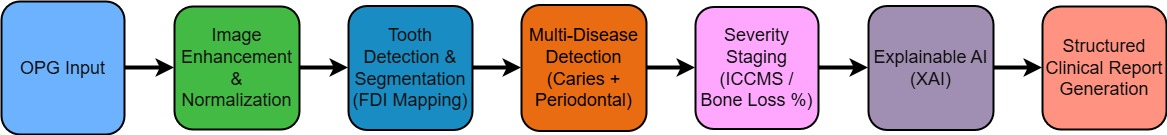
\includegraphics[width=\textwidth]{fig1.jpeg}
    \caption{System Pipeline of Proposed AI Model.}
    \label{fig:pipeline}
\end{figure*}

Furthermore, the lack of standardized datasets and evaluation protocols
limits reproducibility and cross-study comparison. Many studies rely on private, single-center datasets, which introduces dataset bias and poor generalization to external clinical environments \cite{muresanu2024automating,delamare2024panoramic}. Explainable artificial intelligence (XAI) remains rarely used in this domain, despite it's importance for clinical trust,
interpretability, and regulatory acceptance
\cite{ferrara2025applications,bilal2024pdcnet}. The absence of
explainability, combined with inconsistent validation practices, creates
 a substantial barrier to real-world deployment.

Unlike previous surveys that focus on individual tasks or models, this work takes a system-level perspective, analyzing how various components can be integrated into a unified diagnostic framework \cite{zhou2025deep,albano2024artificial}.

We review 47 research papers published between 2021 and 2026 to provide a consolidated view of deep learning methods applied to dental radiograph analysis. The literature is organized into six categories: caries detection and severity classification, periodontal disease and bone loss analysis, multi-task end-to-end diagnosis, explainable AI, dataset benchmarking and clinical validation, and tooth segmentation and numbering. A key finding is that no existing system simultaneously addresses caries detection, severity staging, periodontal bone loss quantification, and explainability within a single unified framework for panoramic radiographs.

The main contributions are as follows:

\begin{itemize}
    \item A task-level taxonomy of deep learning methods for panoramic dental radiograph analysis, covering detection, segmentation, classification, and multi-task architectures.
    \item A problem formulation for unified multi-disease dental diagnosis, highlighting the integration requirements of detection, severity staging, quantification, and explainability.
    \item A comparative analysis of 47 studies, identifying inconsistencies in datasets, evaluation metrics, and validation protocols.
    \item A quantified gap analysis highlighting key limitations in current research, including single-disease focus, lack of automated severity staging, dataset fragmentation, limited use of explainable AI.
    \item A research direction toward clinically deployable, explainable, multi-task dental AI systems.
\end{itemize}

Overall ,this study highlights unified, explainable, multi-task dental AI as an important next step toward clinically deployable diagnostic systems, especially for supporting junior clinicians and dental students .





% -----------------------------------------------------------------------
\section{Search Methodology}
\label{sec:methodology}

This survey used a structured keyword search which was conducted across five digital libraries: IEEE Xplore, PubMed/MEDLINE, Scopus, Google Scholar, and SpringerLink. The search was executed between January 2024 and March 2025, with publication year filters restricting results to 2020 onward.


\subsection{Search Strategy}

Search queries were organized into five thematic clusters:

\begin{itemize}
  \item \textit{Caries detection on panoramic radiographs:}
        ``dental caries'' panoramic radiograph deep learning; ``caries
        detection'' panoramic radiograph CNN; ``caries segmentation''
        orthopantomogram neural network.

  \item \textit{Periodontal disease and bone loss:} ``periodontal
        disease'' panoramic radiograph deep learning; ``alveolar bone
        loss'' orthopantomogram AI; ``CEJ'' ``bone crest'' panoramic
        radiograph segmentation.

  \item \textit{Multi-disease and end-to-end OPG systems:}
        ``multi-task'' dental panoramic radiograph deep learning;
        ``dental disease detection'' panoramic radiograph end-to-end.

  \item \textit{Explainable AI in dental imaging:} ``explainable AI''
        dental radiograph; ``Grad-CAM'' dental panoramic;
        ``interpretable deep learning'' dental imaging.

  \item \textit{Dataset and clinical validation:} ``dental panoramic
        radiograph dataset'' deep learning; ``OPG benchmark'' AI;
        ``clinical validation'' dental AI panoramic.
\end{itemize}

\subsection{Inclusion and Exclusion Criteria}

Papers were included if they: (i)~applied deep learning or machine
learning to dental radiograph analysis; (ii)~used panoramic, bitewing,
or periapical radiographs as primary input; (iii)~targeted detection,
segmentation, classification, or staging of dental caries, periodontal
disease, or related pathologies; and (iv)~reported quantitative
performance metrics. Papers were excluded if they focused exclusively on
CBCT/3D imaging, addressed only non-dental imaging, or did not report
reproducible quantitative results. Clinical reviews without AI models
were included only when they provided foundational clinical definitions
directly relevant to the survey scope.

\subsection{Final Corpus}

After applying the criteria, 47~papers were selected, spanning 2021--2026,
with 25~papers from 2025 (53\%), 17~from 2024 (36\%), 2~from 2026,
2~from 2023, and 1~from 2021 -- reflecting the field's rapid recent
growth. Publication venues include BMC Oral Health (8~papers), IEEE (8),
MDPI journals (9), Elsevier (4), Springer (3), and Scientific
Reports/Nature Portfolio (3).

% -----------------------------------------------------------------------
\section{System-Level Taxonomy and Problem Formulation}
\label{sec:taxonomy}

\subsection{Formal Problem Definition}

Panoramic dental radiograph analysis is inherently a multi-component diagnostic problem that cannot be reduced to single-task prediction. In clinical practice, meaningful diagnosis requires coordinated execution of multiple interdependent processes: anatomical localization of teeth, identification of pathological conditions, assessment of disease severity, and quantitative measurement of clinically relevant parameters. Most existing deep learning systems in the reviewed literature address only one component in isolation
\cite{albano2024artificial,luke2025accuracy,zanini2024systematic},
producing outputs that are diagnostically incomplete and clinically
difficult to integrate.

A unified dental AI system maps an input OPG to structured diagnostic outputs through six core functional components: detection, localization, severity staging, quantification, explainability, and clinical integration. From the reviewed literature, no study in the group of 47 papers addresses all six components simultaneously on panoramic radiographs, identifying a key architectural gap that motivates this survey.

These six core components are defined below:

\begin{itemize}
    \item \textbf{Detection:} Refers to identifying pathological conditions from radiographic features such as carious lesions, periodontal bone loss, periapical pathology, impacted teeth. YOLO-based architectures are used for this task 
          \cite{ayhan2025detection,nassiri2025yolo,chen2024cariesxrays,
          bizjak2024advancing,pornprasertsuk2025clinical}.

    \item \textbf{Localization:}  refers to identifying the position of affected teeth using bounding boxes or segmentation boxes. Tooth level localization using FDI numbering is present in pipeline systems
          \cite{jundaeng2025advanced,chen2024cariesxrays,bizjak2024advancing,
          pornprasertsuk2025clinical} but absent in
          classification-only approaches
          \cite{kaushik2025densenet201,mathur2025comparative,ozdemir2026enhanced}.

    \item \textbf{Severity Staging:} Classification of disease
          progression along clinically meaningful scales. For caries:
          enamel, dentine, pulp involvement
          \cite{asadi2024detection,bizjak2024advancing}. For
          periodontal disease: Stages I--IV per 2018 AAP/EFP
          classification \cite{chmielewski20252018}. This is the most
          critically under addressed component, with only two C1 papers
          providing caries severity differentiation
          \cite{bizjak2024advancing,asadi2024detection}.

    \item \textbf{Quantification:} Measurement of the CEJ--alveolar
          bone crest distance and percentage bone loss. Only three
          studies address this: Jundaeng et al.\ achieved
          mAP50\,=\,0.995 \cite{jundaeng2025advanced}; Wimalasiri et
          al.\ reported ICC\,=\,0.80 \cite{wimalasiri2025ai}; and Tian
          et al.\ achieved ICC\,=\,0.83 \cite{tian2025development}.

    \item \textbf{Explainability:} Generation of interpretable visual
          outputs for clinical verification. Only 3 of 47 papers
          implement explainability (6.4\%): Chen et al.\
          \cite{chen2023deep} and Bilal et al.\ \cite{bilal2024pdcnet}
          use Grad-CAM, and Chen et al.\ \cite{chen2024cariesxrays}
          show feature map attention.

    \item \textbf{Clinical Integration:} Alignment with diagnostic
          workflows, reporting standards, and regulatory requirements.
          Only Schwendicke et al.\ \cite{schwendicke2021cost} model
          economic impact, and only Lee et al.\ \cite{lee2025evaluation}
          measure clinician acceptance through a 65-dentist usability
          survey.
\end{itemize}

This six-component formulation stands in direct contrast to existing
approaches that address each task in isolation -- a fragmentation
independently identified as critical by multiple systematic reviews
\cite{iacob2025automated,albano2024artificial,bonfanti2025deep,
khubrani2025detection,zanini2024systematic,zhou2025deep}.

\subsection{System Taxonomy}

Existing approaches are grouped into four system archetypes based on task integration and diagnostic scope. This taxonomy shows both progress toward integration and the limitations that fully prevent full clinical use. Table~\ref{tab:taxonomy} summarizes the capability coverage across these categories.

\subsubsection{Single-Task Approaches}

Single-task systems focus on one diagnostic objective, such as, caries detection, tooth segmentation, or periodontal classification – without integration. This accounts for most reviewed studies (18 C1, 15 C2 papers). While several studies report high performance, such as CariesXrays FPCL reaching AP50\,=\,84.1\% \cite{chen2024cariesxrays},
Attention U-Net achieving Recall\,=\,0.96
\cite{pornprasertsuk2025clinical}, U-Net variants reporting
Dice\,=\,96.77\% \cite{vickram2025extraction} -- none produce severity
grading, periodontal assessment, or clinical explanations. The main limitation is not performance but scope, as these models focus on a single task without considering interactions with other diagnostic tasks. This is also supported by systematic reviews
\cite{albano2024artificial,zanini2024systematic}, which highlights the lack of multi-task integration as the key limitation.

\subsubsection{Multi-Task Approaches}

Seven studies explore multi-task designs with varying completeness. Chen et al.\ \cite{chen2023deep} is one of the more complete approaches, classifying both periodontitis and caries on a per-tooth basis using EfficientNetB0 with YOLOv7 localization  (ROC AUC\,=\,98.67\% for periodontitis, 98.31\% for caries) with Grad-CAM
explainability. However, this system operates exclusively on periapical
radiographs -- not panoramic OPGs -- which limits its direct applicability to panoramic radiographs. Multi-task approaches shows a clear performance difference: structural tasks (such as segmentation and enumeration) achieve high accuracy, while pathological tasks (such as disease detection and severity staging) remain more challenging. Mure\c{s}anu et al.\
\cite{muresanu2024automating} reported that: YOLOv8
F1 dropped from 0.60 (internal) to 0.47 (external) -- a 22\%
decrease due to single-center training.

\subsubsection{Pipeline-Based Approaches}

Pipeline-based systems break the diagnosis process into sequential stages like similar to how clinicians approach diagnosis. Jundaeng et al.\
\cite{jundaeng2025advanced} implemented a precise periodontal pipeline:
YOLOv8 Stage~1 for tooth segmentation (mAP50\,=\,0.92) feeds Stage~2
for CEJ and bone crest detection (mAP50\,=\,0.995,
Sensitivity\,=\,1.0). Pornprasertsuk-Damrongsri et al.\
\cite{pornprasertsuk2025clinical} combined YOLOv5s for tooth detection
with Attention U-Net for caries segmentation (Recall\,=\,0.96,
F1\,=\,0.85). A key limitation is error propagation where mistakes in early stages affect later stages. None of the reviewed pipelines address severity staging, and explainability appear only in one system \cite{chen2023deep} -- which operates on periapical rather than panoramic, radiographs.

\subsubsection{End-to-End Approaches}

End-to-end models map radiographs to diagnostic outputs using deep architectures, primarily transformer-based models. Bhoopalan et al.\
\cite{bhoopalan2026self} applied Vision Transformer (ViT) and Swin Transformer
to 5,098 OPGs, achieving ViT accuracy\,=\,96\% without spatial
localization or severity grading. Van Nistelrooij et al.\
\cite{vannistelrooij2024combining} combined multiple datasets and transformer-based architectures to improve tooth-level analysis, although computational complexity and inference time remain challenges. The fundamental barrier is data: the field lacks large-scale, multi-disease, multi-center public datasets required for end-to-end learning.

The system-level taxonomy and capability gaps across different architectural paradigms are illustrated in Fig.~\ref{fig:taxonomy}

\begin{figure*}[t]
  \centering
  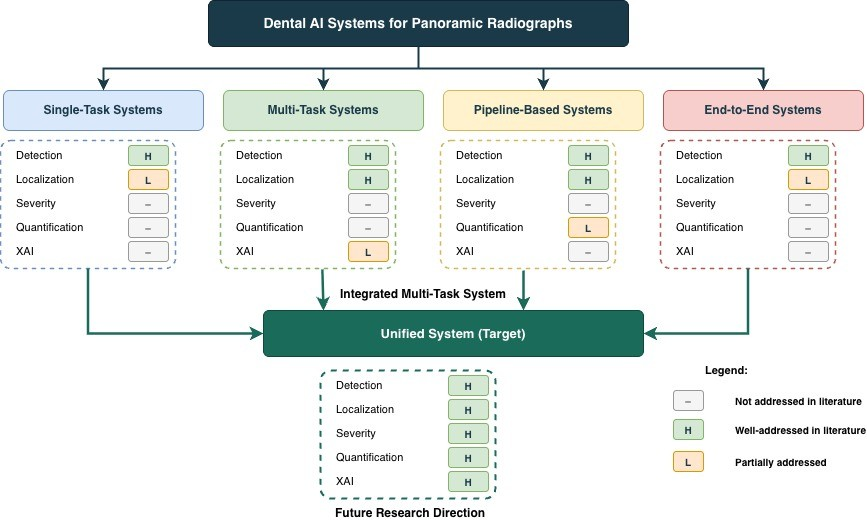
\includegraphics[width=0.85\textwidth]{fig4.jpeg}
  \caption{System-level taxonomy of dental AI approaches for panoramic radiographs, 
  illustrating four architectural paradigms (Single-Task, Multi-Task, Pipeline-Based, 
  and End-to-End Systems) and their respective capability coverage across detection, 
  localization, severity, quantification, and explainability (XAI) dimensions, 
  alongside the proposed Unified System as a future research direction.}
  \label{fig:taxonomy}
\end{figure*}

\begin{table*}[t]
\renewcommand{\arraystretch}{1.5}
\caption{System Taxonomy --- Representative Studies by Design Pattern
and Capability Coverage}
\label{tab:taxonomy}
\centering
\scriptsize
\setlength{\tabcolsep}{4pt}
\begin{tabular}{p{1.6cm} p{3.5cm} p{1.0cm} p{1.2cm} p{1.2cm} p{1.0cm} p{1.0cm} p{1.5cm}}
\toprule
\textbf{System Type} & \textbf{Representative Studies} &
\textbf{Detect} & \textbf{Localize} & \textbf{Severity} &
\textbf{Quant.} & \textbf{XAI} & \textbf{Multi-Disease} \\
\midrule
Single-Task &
\cite{ayhan2025detection,alharbi2023detection,khuwaja2024ai,
chen2024cariesxrays,perez2024ai,zancan2025ai,ozdemir2026enhanced}
& \checkmark & Partial & \texttimes & \texttimes & \texttimes & \texttimes \\

Multi-Task &
\cite{nassiri2025yolo,chen2023deep,gamal2025automated,
vannistelrooij2024combining,muresanu2024automating,bhoopalan2026self}
& \checkmark & \checkmark & \texttimes & \texttimes & Partial & Partial \\

Pipeline-Based &
\cite{jundaeng2025advanced,chen2024cariesxrays,bizjak2024advancing,
pornprasertsuk2025clinical}
& \checkmark & \checkmark & \texttimes & Partial & \texttimes & \texttimes \\

End-to-End &
\cite{vannistelrooij2024combining,bhoopalan2026self}
& \checkmark & Partial & \texttimes & \texttimes & \texttimes & Partial \\

\midrule
\textbf{Unified (Required)} & \textit{None in reviewed corpus}
& \checkmark & \checkmark & \checkmark & \checkmark & \checkmark & \checkmark \\
\bottomrule
\multicolumn{8}{l}{\footnotesize \checkmark\,=\,fully addressed;\
\texttimes\,=\,not addressed;\ Partial\,=\,partially addressed.}\\
\multicolumn{8}{l}{\footnotesize Quant.\,=\,quantitative measurement;\
XAI\,=\,explainable AI outputs.}\\
\end{tabular}
\end{table*}

\subsection{Task Hierarchy}

Dental radiograph analysis follows a structured sequence of
interdependent processing stages reflecting the actual cognitive process
trained clinicians employ:

\begin{figure*}[t]
  \centering
  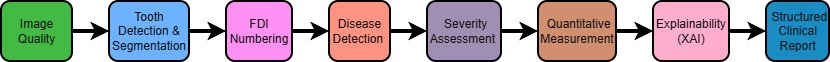
\includegraphics[width=0.95\textwidth]{fig5.jpeg}
  \caption{Task hierarchy for panoramic dental radiograph analysis, showing stages from anatomical structure extraction to clinical report generation. Early stages, such as tooth segmentation and numbering, usually perform well. However, later stages like severity assessment, quantification, and explainability are less explored, which highlights current limitations.}
  \label{fig:taskhierarchy}
\end{figure*}

Early stages focus on anatomical structure identification, where systems
perform well: tooth segmentation achieves pooled sensitivity\,=\,0.92,
specificity\,=\,0.94 \cite{bonfanti2025deep}; tooth enumeration reaches
mAP50\,=\,0.978 \cite{nassiri2025yolo}. Middle stages -- disease
detection and severity assessment -- represent the performance
bottleneck. Disease detection on OPG reaches only mAP50\,$\approx$\,0.61
\cite{nassiri2025yolo}, and severity staging is attempted in only two
of 18 C1 papers \cite{bizjak2024advancing,asadi2024detection}. Terminal
stages -- explainability and structured reporting -- are most neglected:
explainability appears in only 3 of 47 papers (6.4\%)
\cite{chen2023deep,chen2024cariesxrays,bilal2024pdcnet}, and structured
report generation is absent from all systems. This hierarchy shows that dental AI is a sequential reasoning problem, where failures in early stages can affect downstream diagnostic decisions. For systems targeting junior clinicians, the absence of visual explanations reduces its educational value.

\subsection{System-Level Limitations}

Five system-level limitations persist across the reviewed literature,
reflecting field-wide methodological choices:

\begin{itemize}
    \item \textbf{Task Fragmentation:} No panoramic OPG system
          simultaneously addresses caries detection, severity staging,
          periodontal quantification, and explainability. Chen et al.\
          \cite{chen2023deep} achieves dual-disease detection with
          explainability -- closest to unified -- but only on periapical
          radiographs.

    \item \textbf{Severity Staging Deficit:} Only Asadi
          \cite{asadi2024detection} and Bizjak and Robic
          \cite{bizjak2024advancing} provide caries severity
          differentiation among 18 C1 papers. For periodontal disease,
          the 2018 AAP/EFP Stages I--IV \cite{chmielewski20252018} are
          not addressed by existing systems.

    \item \textbf{Limited Explainability:} Only 3 of 47 papers
          implement explainability (6.4\%), despite a general consensus in the field
          \cite{nassiri2025yolo,gamal2025automated,sastika2025ai,
          ferrara2025applications,khubrani2025detection}. The EU AI Act
          and FDA guidance require transparency for high-risk systems --
          requirements 43 of 47 systems do not satisfy.

    \item \textbf{Dataset Fragmentation:} Approximately 60\% of studies
          use private, single-center datasets which lead to heterogeneity
          values $I^2$\,=\,88--96\%
          \cite{iacob2025automated,albano2024artificial,bonfanti2025deep}.
          Mure\c{s}anu et al.\ \cite{muresanu2024automating} documented
          22\% F1 degradation from internal to external data. There is currently no large-scale, multi-disease, multi-center, publicly available panoramic dataset with standardized annotations.

    \item \textbf{Clinical Workflow Disconnection:} With the exception of 
          Schwendicke et al.\ \cite{schwendicke2021cost}
          (cost-effectiveness analysis) and Lee et al.\
          \cite{lee2025evaluation} (65-dentist usability study), no system evaluates AI within actual clinical workflows. Most systems produce outputs such as bounding boxes without structured reports or treatment recommendations..
\end{itemize}
%---------------------------

\section{Background}
\label{sec:background}

\subsection{Panoramic Radiography in Clinical Dentistry}

Orthopantomography (OPG) produces a two-dimensional representation of the curved dental arches on a flat image plane. Unlike periapical or bitewing radiographs that show specific regions, a single panoramic image captures all 32 permanent teeth, maxilla and mandible, and surrounding structures -- making it one of the most informative radiographic methods in routine dental practice. For caries detection, panoramic radiographs are less sensitive than bitewing images for early proximal lesions \cite{perez2024ai,bizjak2024advancing,pornprasertsuk2025clinical}.
For periodontal bone loss assessment, OPG is commonly used as a screening
tool, as it allow visualization of the alveolar crest relative to the
cemento-enamel junction (CEJ) across all teeth
\cite{jundaeng2025advanced,iacob2025automated,khubrani2025detection}.
This difference in imaging affects how AI systems are designed for each task.

\subsection{Deep Learning Architectures}

The architectures reviewed can be divided into four major categories. First,
CNNs with transfer learning, such as ResNet~\cite{khuwaja2024ai},
DenseNet~\cite{kaushik2025densenet201,ozdemir2026enhanced},
VGG~\cite{mathur2025comparative}, EfficientNet~\cite{chen2023deep},
Inception~\cite{gamal2025automated,zancan2025ai}  are mostly used for classification tasks, These models often use ImageNet pre-training because dental datasets are limited. Second, YOLO-family one-stage object
detectors (YOLOv5--YOLOv9)
\cite{ayhan2025detection,nassiri2025yolo,bizjak2024advancing,muresanu2024automating,pornprasertsuk2025clinical} are widely used for detection tasks owing to their speed and accurate bounding box localization. Third U-Net variants 
\cite{alharbi2023detection,asci2024deep,lim2024dual,kong2024integrating,zanini2024systematic}
are used for pixel-level segmentation, where skip connections help preserve fine spatial details. Fourth, transformer architectures -- ViT
\cite{bhoopalan2026self}, Swin Transformer
\cite{vannistelrooij2024combining,zhang2025reliable}, RT-DETR
\cite{karamuftuo2025panoramic} -- represent newer approaches offering global attention but at higher computational cost.

\subsection{Evaluation Metrics}

A persistent challenge across the reviewed literature is metric
inconsistency that prevents direct cross-study comparison
\cite{iacob2025automated,bonfanti2025deep,khubrani2025detection,zanini2024systematic}.
Object detection studies report mAP at IoU thresholds of 0.50 and
0.50:0.95. Segmentation studies report IoU and Dice coefficient.
Classification studies report accuracy, AUC, sensitivity, specificity,
and F1. Several studies \cite{chen2023deep,bilal2024pdcnet,zancan2025ai}
additionally report PPV and NPV -- metrics with direct clinical
relevance that standard accuracy obscures. The absence of a standardized
dental AI evaluation protocol is identified as one of the field's most
critical methodological gaps
\cite{iacob2025automated,luke2025accuracy,khubrani2025detection}.

% -----------------------------------------------------------------------
\section{Caries Detection and Severity Classification (C1)}
\label{sec:caries}

Caries detection is the most extensively studied task in dental AI, accounting for 18 of the 47 reviewed papers.
These Studies cover object detection, segmentation, classification, and systematic review methodologies across panoramic, bitewing, periapical, and intraoral RGB modalities.


\subsection{YOLO-Based Detection on Panoramic Radiographs}

Ayhan et al.~\cite{ayhan2025detection} proposed a two-stage pipeline for detecting caries beneath fixed dental prostheses (FDPs) -- a clinically challenging scenario where metal artifacts from crowns and bridges can obscure lesion visibility. YOLOv7 was used to detect FDP regions
(mAP\,=\,0.968, F1\,=\,0.956) in Stage~1; a CBAM-enhanced YOLOv7
applied to cropped ROIs achieved caries detection with mAP\,=\,0.846
and F1\,=\,0.830 in Stage~2. The CBAM attention module improved detection of low-contrast lesion boundaries beneath metallic
artifacts.

Bizjak and Robic~\cite{bizjak2024advancing} used a two-step YOLOv8
pipeline on the public DENTEX dataset, achieving tooth enumeration
mAP@0.5\,=\,0.95 and lesion sensitivity\,=\,0.70 (internal), 0.67
(external) -- This is one of the few studies that includes external clinical validation, showing performance degradation from internal to external data. Asadi~\cite{asadi2024detection} used Faster
R-CNN on the UFBA-UESC public dataset, achieving 94\% overall accuracy
and reported an important limitation: recall for mild
caries\,=\,0.64 versus severe caries\,=\,0.69 -- which is not ideal in practice, since early lesions are more important to detect.
Pornprasertsuk-Damrongsri et al.~\cite{pornprasertsuk2025clinical}
combined YOLOv5s for tooth detection with Attention U-Net for caries
segmentation on 500 panoramic radiographs with bitewing-confirmed ground
truth, achieving Recall\,=\,0.96, F1\,=\,0.85 with Bland-Altman
agreement analysis.An example of multi-tooth carious lesion detection with severity differentiation in panoramic radiographs is shown in Fig.~\ref{fig:dentex} .

\begin{figure*}[t]
    \centering
    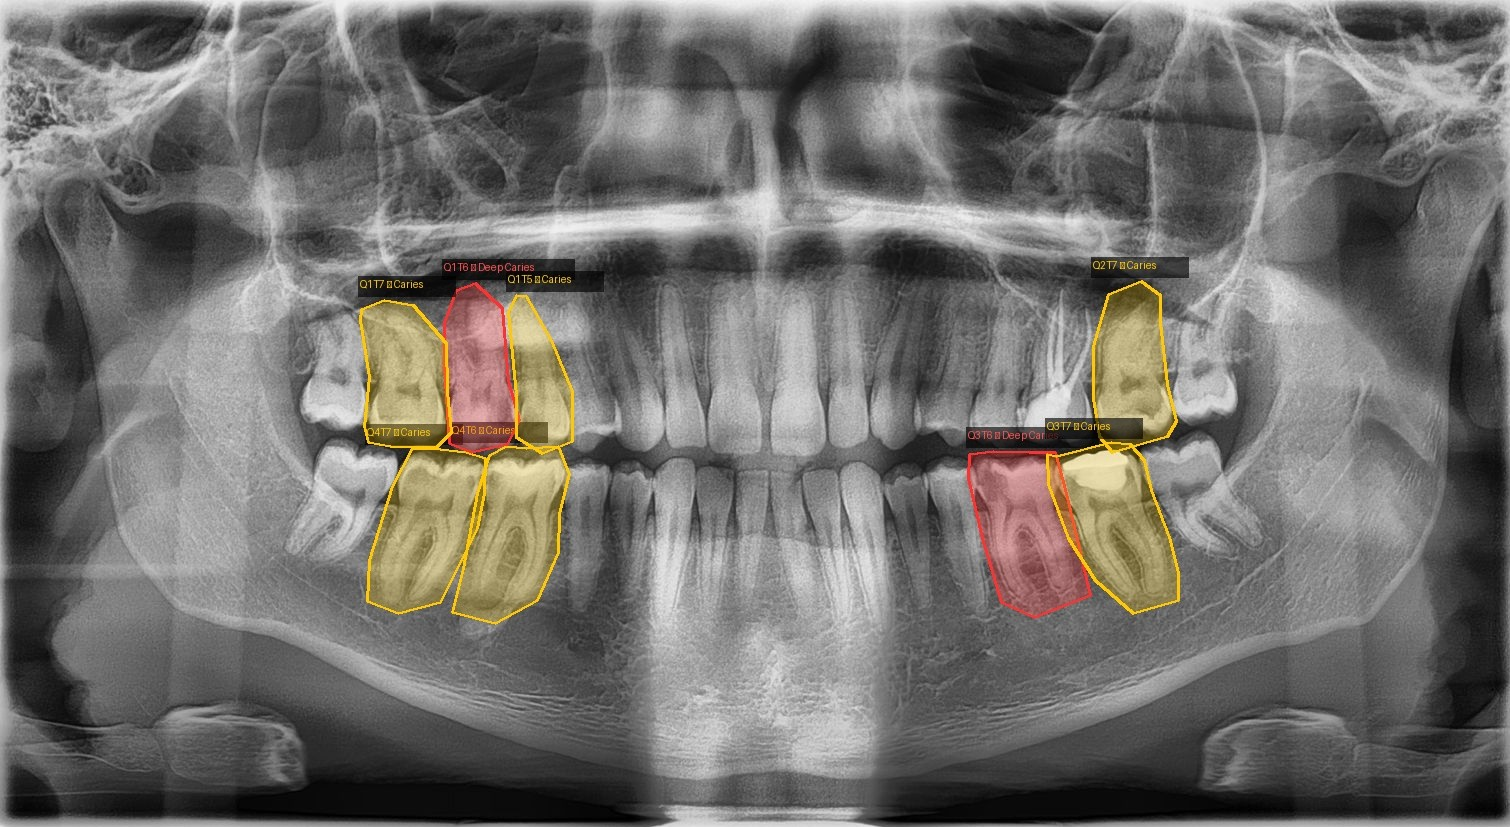
\includegraphics[width=0.65\textwidth]{fig2.jpg}
    \caption{Example panoramic radiograph with annotated carious lesions, 
    illustrating multi-instance detection and severity differentiation 
    (caries vs.\ deep caries) across multiple teeth.}
    \label{fig:dentex}
\end{figure*}

\subsection{U-Net Segmentation Approaches}

Alharbi et al.~\cite{alharbi2023detection} compared U-Net, U-Net++, and
U-Net3+ on 1,500 panoramic images. U-Net3+ achieved the best test
performance (IoU\,=\,0.67, Dice\,=\,0.60, Accuracy\,=\,0.95), with its
full-scale skip connections providing measurable advantage over standard
U-Net (Dice\,=\,0.58). The gap between training IoU (0.77) and test IoU
(0.67) reveals overfitting from severe class imbalance -- only 510 of
1,500 images contained visible cavities.

Lim et al.~\cite{lim2024dual} proposed Faster R-CNN + U-Net
(EfficientNet-B0 encoder) on 597 panoramic radiographs, achieving
IoU\,=\,0.608, Dice\,=\,0.743, Recall\,=\,0.731 on 33,752 augmented
cropped tooth images, though without severity grading or explainability.
Asci et al.~\cite{asci2024deep} applied U-Net to 6,075 pediatric
panoramic radiographs stratified across primary, mixed, and permanent
dentition, achieving F1\,=\,0.8675, Sensitivity\,=\,0.8269,
Precision\,=\,0.9123 -- demonstrating U-Net's adaptability across
diverse tooth morphologies, though AUC\,=\,0.76 remains below the 90\%
clinical threshold. Vickram and Mathan Muthu~\cite{vickram2025extraction}
applied UNet variants on 500 dental X-ray images, achieving
Accuracy\,=\,98.03\% and Dice\,=\,96.77\%, though on a notably small
dataset with no clinical validation.


\subsection{CNN Classification and Transfer Learning}

Zancan et al.~\cite{zancan2025ai} applied InceptionResNet-v2 to 7,304
tooth-level images from 935 panoramic radiographs, achieving
accuracy\,=\,0.94 and F1\,=\,0.94 with five-fold cross-validation --
one of the stronger validation approaches in C1. Kaushik and
Sharma~\cite{kaushik2025densenet201} applied DenseNet201 to 29,815
dental X-ray images, achieving 91\% overall accuracy but a
cavity-specific F1 of only 0.27 -- a stark illustration of class
imbalance consequences. Ozdemir et al.~\cite{ozdemir2026enhanced}
applied DenseNet-121 to 14,498 cropped tooth images (2,303 caries /
12,195 non-caries), achieving accuracy\,=\,93.17\% and F1\,=\,87.49\%,
though without localization on full panoramic images. Khuwaja et
al.~\cite{khuwaja2024ai} evaluated YOLOv8, ResNet-50, EfficientDet, and
MobileNetV2 on 7,447 intraoral RGB smartphone images -- targeting mobile
diagnostics for resource-limited settings -- with ResNet-50 achieving
mAP@0.50\,=\,0.670.

\subsection{Systematic Reviews and Meta-Analyses}

Albano et al.~\cite{albano2024artificial} reviewed 20 studies via
PRISMA/QUADAS-2, finding accuracy 73\%--98\% and AUC 0.84--0.98 across
CNN-based models, with high heterogeneity and an explicit call for
standardized datasets and multicenter validation. Luke and
Rezallah~\cite{luke2025accuracy} conducted a meta-analysis of 21 studies
(17,190 total samples), reporting the best individual study achieving
98.8\% accuracy but $I^2$ values of 88--96\% indicating severe
heterogeneity that undermines pooled estimates. Zanini et
al.~\cite{zanini2024systematic} reviewed 42 studies confirming that most
works are single-task and lack caries severity differentiation as a
systematic field-wide gap. Sastika and Marappan~\cite{sastika2025ai}
reviewed accuracy ranges of 85--99\% across multiple architectures,
notably acknowledging Grad-CAM as a requirement in surveyed studies.

Chen et al.~\cite{chen2024cariesxrays} introduced the CariesXrays
dataset (6,000 hospital-grade panoramic X-rays, 13,783 expert-verified
bounding boxes) alongside the FPCL architecture -- achieving
AP\,=\,48.2\%, AP50\,=\,84.1\%, outperforming YOLOv8
(AP50\,=\,80.7\%). CariesXrays is the most significant public benchmark
contribution in the C1 category.

\subsection{Bitewing Caries and Cost-Effectiveness}

Perez de Frutos et al.~\cite{perez2024ai} evaluated RetinaNet,
YOLOv5-M, and EfficientDet on 13,887 bitewing X-rays from the HUNT4
Oral Health Study, annotated by six dentists with a 197-image consensus
test set. YOLOv5-M achieved mAP\,=\,0.647, F1\,=\,0.548 -- matching or
surpassing individual expert annotators, providing strong evidence that
deep learning performs at human expert level on proximal caries
detection. Schwendicke et al.~\cite{schwendicke2021cost} combined U-Net
performance evaluation (accuracy\,=\,0.80, sensitivity\,=\,0.75 vs.\
dentist sensitivity\,=\,0.36) with a Markov lifetime cost-effectiveness
simulation on 3,686 bitewing radiographs, projecting increased tooth
retention (64 vs.\ 62 years) and reduced cost per tooth
(\euro298 vs.\ \euro322), yielding ICER\,=\,$-$13.9~\euro/year --
establishing AI caries detection as a cost-dominant strategy.

\begin{table*}[t]
\caption{Summary of Reviewed Studies --- Caries Detection and Severity Classification (C1)}
\label{tab:c1}
\centering
\small
\begin{tabular}{p{0.6cm} p{4.8cm} p{3.0cm} p{3.5cm} p{1.0cm} p{3.2cm}}
\toprule
\textbf{Ref} & \textbf{Model} & \textbf{Dataset Size} & \textbf{Best Metric} & \textbf{XAI} & \textbf{Key Gap} \\
\midrule
\cite{ayhan2025detection}   & YOLOv7 + CBAM & 1,004 OPG & mAP=0.846, F1=0.830 & None & Single-center, no XAI \\
\cite{khuwaja2024ai}        & YOLOv8, ResNet-50, EfficientDet, MobileNetV2 & 7,447 RGB & mAP@0.50=0.670 & None & RGB only, no radiographs \\
\cite{alharbi2023detection} & U-Net, U-Net++, U-Net3+ & 1,500 OPG & IoU=0.67, Dice=0.60 & None & Class imbalance, no severity \\
\cite{asci2024deep}         & U-Net & 6,075 OPG (pediatric) & F1=0.8675, AUC=0.76 & None & Below 90\% clinical threshold \\
\cite{albano2024artificial} & Systematic Review (CNNs) & 20 studies & Acc up to 0.98, AUC 0.98 & None & High heterogeneity \\
\cite{kaushik2025densenet201} & DenseNet201 & 29,815 X-rays & Acc=91\%, Cavity F1=0.27 & None & Severe class imbalance \\
\cite{chen2024cariesxrays}  & FPCL (Faster R-CNN + D2D-FPN + Contrastive) & 6,000 OPG & AP=48.2\%, AP50=84.1\% & Attn maps & No severity/periodontal \\
\cite{perez2024ai}          & YOLOv5-M, RetinaNet, EfficientDet & 13,887 bitewing & mAP=0.647, F1=0.548 & None & Bitewing only, no periodontal \\
\cite{sastika2025ai}        & Review: U-Net, ResNet, YOLOv7/v8, ensemble & Multiple studies & Acc 85--99\%, F1 87--94\% & Discussed & No original experiment \\
\cite{schwendicke2021cost}  & U-Net & 3,686 bitewing & Acc=0.80, ICER=$-$\euro13.9/yr & None & Single-center, German context \\
\cite{luke2025accuracy}     & Meta-analysis (CNNs) & 21 studies, 17,190 images & Best Acc=98.8\% & None & $I^2$=88--96\% heterogeneity \\
\cite{vickram2025extraction}& UNet, UNet+, UNet++ & 500 images & Acc=98.03\%, Dice=96.77\% & None & Small dataset, no clinical val. \\
\cite{zancan2025ai}         & InceptionResNet-v2 & 935 OPG / 7,304 teeth & Acc=0.94, F1=0.94 & None & No localization, no periodontal \\
\cite{lim2024dual}          & Faster R-CNN + U-Net (EfficientNet-B0) & 597 OPG & IoU=0.608, Dice=0.743 & None & No severity, no periodontal \\
\cite{zanini2024systematic} & Systematic Review (U-Net, Mask R-CNN, ResNet) & 42 studies & Various (review) & None & No severity differentiation \\
\cite{bizjak2024advancing}  & YOLOv8 two-step pipeline & 1,005 OPG + 85 external & mAP@0.5=0.95, Sens=0.70 & None & Caries only, no severity \\
\cite{asadi2024detection}   & Faster R-CNN & 1,000 OPG & Acc=94\%, Mild recall=0.64 & None & Weak mild caries detection \\
\cite{pornprasertsuk2025clinical} & YOLOv5s + Attention U-Net & 500 OPG, 14,997 teeth & Recall=0.96, F1=0.85 & None & Single-disease, no periodontal \\
\cite{ozdemir2026enhanced}  & DenseNet-121 & 14,498 tooth images & Acc=93.17\%, F1=87.49\% & None & No localization, no severity \\
\bottomrule
\end{tabular}
\end{table*}

% -----------------------------------------------------------------------
\section{Periodontal Disease and Alveolar Bone Loss Detection (C2)}
\label{sec:perio}

Periodontal disease detection from radiographs requires quantifying the
spatial relationship between anatomical landmarks -- specifically the
distance between the cemento-enamel junction (CEJ) and the alveolar
bone crest -- across all teeth in the panoramic image. This requires precise spatial localization and continuous measurement rather than binary classification. Fifteen papers in the C2 category indicate that this area is still developing but progressing rapidly.

\subsection{Clinical Foundation}

Chmielewski et al.~\cite{chmielewski20252018} provide essential clinical
framing: the 2018 AAP/EFP classification defines periodontitis
stages~I--IV and grades~A--C based on bone loss percentage, probing
depth, tooth loss, and risk factors. Across 11 clinical studies covering
459 cases and 852 examiners, staging accuracy peaked at 90\% but
inter-examiner agreement remained variable -- a subjectivity problem
that AI systems can address, but only if they produce quantitative,
staged outputs aligned with the 2018 criteria rather than binary bone
loss labels. Fig.~\ref{fig:perio} illustrates the spatial nature of periodontal bone loss assessment, requiring accurate identification of anatomical landmarks such as the cemento-enamel junction and alveolar bone crest.

\begin{figure*}[t]
    \centering
    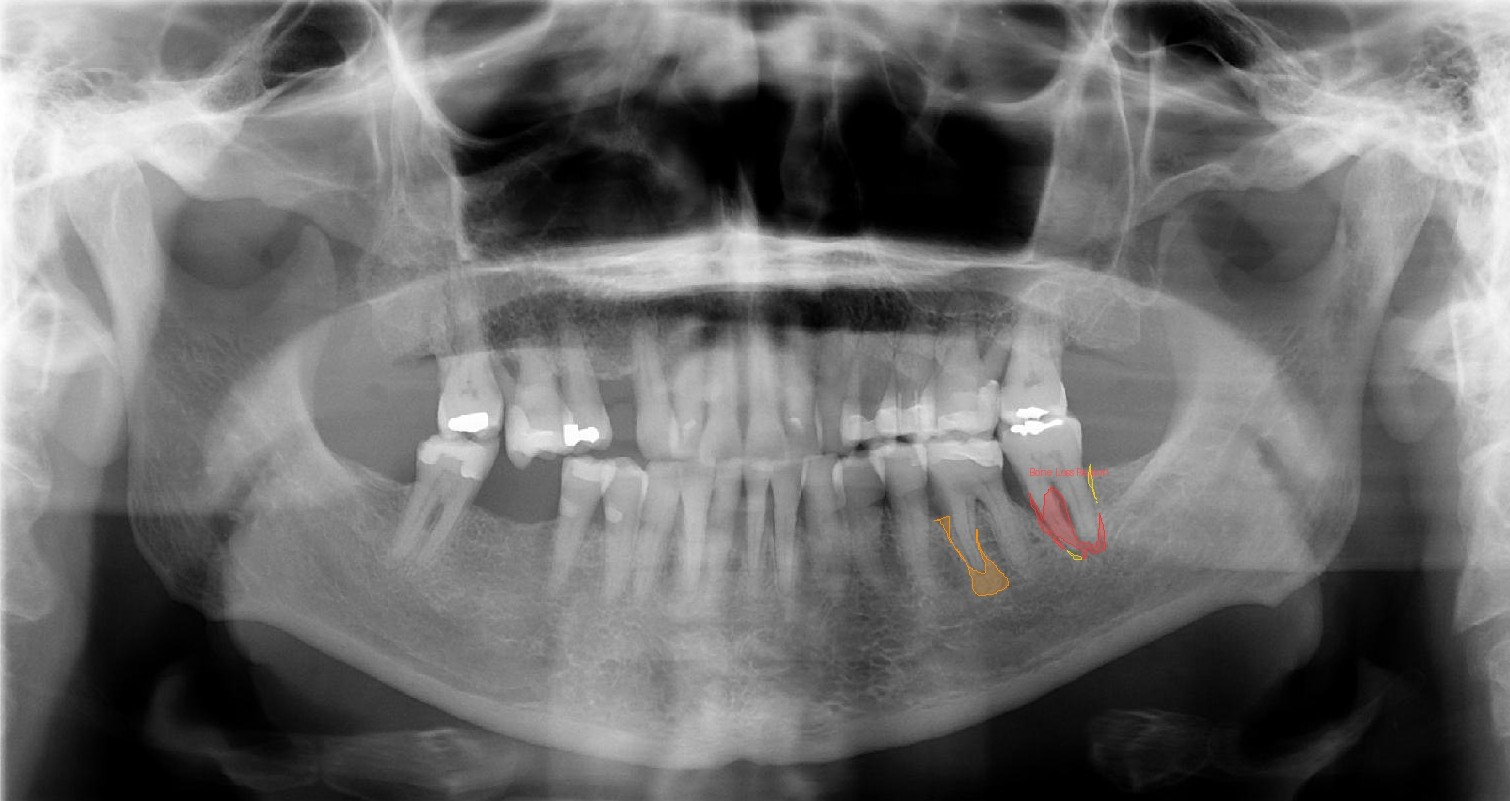
\includegraphics[width=0.65\textwidth]{fig3.jpg}
    \caption{Example panoramic radiograph illustrating periodontal bone 
    loss regions. Accurate assessment requires spatial measurement between 
    the cemento-enamel junction and alveolar bone crest.}
    \label{fig:perio}
\end{figure*}

\subsection{Landmark Detection and Bone Loss Quantification}

Jundaeng et al.~\cite{jundaeng2025advanced} presented the most
technically complete periodontal AI system reviewed. Their dual YOLOv8
pipeline on 2,000 panoramic radiographs achieved tooth segmentation
(Accuracy\,=\,0.97, mAP50\,=\,0.92) and CEJ/bone level detection
(Accuracy\,=\,0.98, Sensitivity\,=\,1.0, Specificity\,=\,0.98,
F1\,=\,0.90, mAP50\,=\,0.995). Sensitivity\,=\,1.0 for bone level
detection carries real clinical importance -- in a screening context ,failing to identify true bone loss is more
harmful than a false positive . Limitations
include single-center data, high-quality images only, and no caries
integration or explainability.

Iacob et al.~\cite{iacob2025automated} synthesized evidence from 20
diagnostic accuracy studies covering 141,166 radiographs through
PRISMA/QUADAS-2, finding that U-Net, YOLO, ResNet, ConvNeXt, and
DeNTNet have all been applied but high heterogeneity prevents reliable
pooling. Khubrani et al.~\cite{khubrani2025detection} meta-analyzed 30
studies using APPRAISE-AI, reporting pooled sensitivity\,=\,87\%,
specificity\,=\,76\%, accuracy\,=\,84\% -- useful but insufficient for
autonomous clinical use.

Mathur et al.~\cite{mathur2025comparative} applied VGG-16 to 1,874
panoramic radiographs for binary bone loss classification
(accuracy\,=\,89.27\%, sensitivity\,=\,83.27\%) -- the most common C2
approach but also the most clinically limited, providing no staging
information. Cerda Mardini et al.~\cite{cerda2024determining} attempted
quantitative staging on 500 panoramic radiographs, reporting
F1\,=\,0.29 for light-moderate bone loss and F1\,=\,0 for severe bone
loss -- honestly documenting the difficulty of quantitative staging and
the model's failure on the most clinically critical class. Kong et
al.~\cite{kong2024integrating} integrated SRGAN super-resolution
preprocessing with U-Net for bone loss segmentation
(Dice\,=\,0.91, IoU\,=\,84.9\%) -- the strongest segmentation metrics
in C2 -- demonstrating that preprocessing quality directly impacts
segmentation accuracy, though the dataset of 698 images is small and no
disease staging is provided.

Wimalasiri et al.~\cite{wimalasiri2025ai} applied YOLOv8x and Keypoint
R-CNN to 1,000 intraoral periapical X-rays, achieving ICC\,=\,0.80 for
severity and 87\% for bone loss pattern classification (horizontal
vs.\ vertical) -- the only study addressing pattern classification,
which has direct prognostic implications for surgical planning. Tian et
al.~\cite{tian2025development} developed the PAN-POL mathematical model
validated on 290 panoramic patients, achieving ICC\,=\,0.83, though
this is a rule-based approach rather than a deep learning system.

\subsection{Periodontitis Classification}

Bilal et al.~\cite{bilal2024pdcnet} proposed PDCNET -- a custom
five-block CNN with Grad-CAM explainability -- compared against
EfficientNet-B0, DenseNet-201, VGG-16, VGG-19, Inception-V3, and
MobileNet on a Kaggle dataset augmented with SMOTE-Tomek, achieving
accuracy\,=\,98.39\%, AUC\,=\,99.79\%, F1\,=\,98.31\%. These are the
highest classification metrics in C2, though the 50+50 original sample
size raises serious concerns about statistical meaningfulness. The paper
is valuable for demonstrating Grad-CAM feasibility in periodontal AI.
Ferrara et al.~\cite{ferrara2025applications} reviewed 13 periodontal
deep learning studies via PRISMA/QUADAS-2, reporting accuracy ranges of
73\%--98.6\% and noting the complete absence of explainable AI across
reviewed systems. Lee et al.~\cite{lee2025evaluation} evaluated AI
alveolar bone loss measurement usability through a survey of 65 dentists
on 550 bitewing images -- one of the only clinical usability studies in
the entire reviewed corpus.

Kim et al.~\cite{kim2024unsupervised} proposed an unsupervised few-shot
learning architecture combining UNet, CVAE, and clustering methods
(k-means/DBSCAN/GMM) on 1,372 panoramic radiographs, achieving a 14\%
improvement over supervised ViT, demonstrating the potential of
label-efficient learning in data-scarce dental AI settings.
Karamuftuo\u{g}lu et al.~\cite{karamuftuo2025panoramic} benchmarked
YOLOv12x, RT-DETR-L, and RT-DETR-X on a 387-image pediatric panoramic
dataset for furcation lesion detection, achieving mAP@0.5\,=\,0.434 --
reflecting both the difficulty of the task and the limitation of small
single-center datasets.

\begin{table*}[t]
\caption{Summary of Reviewed Studies --- Periodontal Disease and Bone Loss (C2)}
\label{tab:c2}
\centering
\small
\begin{tabular}{p{0.6cm} p{4.5cm} p{3.0cm} p{3.8cm} p{1.0cm} p{2.8cm}}
\toprule
\textbf{Ref} & \textbf{Model} & \textbf{Dataset Size} & \textbf{Best Metric} & \textbf{XAI} & \textbf{Key Gap} \\
\midrule
\cite{jundaeng2025advanced}  & Dual YOLOv8 (teeth + CEJ/bone) & 2,000 OPG & mAP50=0.995, Sens=1.0 & None & Single-center, no caries \\
\cite{chmielewski20252018}   & Clinical review (no ML) & 459 cases, 852 examiners & Stage acc=90\% & None & No AI system proposed \\
\cite{iacob2025automated}    & Systematic Review (CNN, YOLO, U-Net) & 141,166 radiographs & Various (review) & None & High heterogeneity \\
\cite{mathur2025comparative} & VGG-16 (transfer learning) & 1,874 OPG & Acc=89.27\% & None & Binary only, no staging \\
\cite{khubrani2025detection} & Meta-analysis (CNN, YOLO, U-Net, SVM) & 30 studies & Sens=87\%, Spec=76\% & None & Pooled heterogeneity \\
\cite{tian2025development}   & PAN-POL mathematical model & 290 PAN patients & ICC=0.83 & None & Not deep learning, manual \\
\cite{lee2025evaluation}     & Faster R-CNN + DeepLab v3+ & 550 bitewing & Acc=82--87\% (severe) & None & Bitewing only, no OPG \\
\cite{cerda2024determining}  & Hybrid DCNN (Xception) + rule-based PBL & 500 OPG & F1=0.29 (lt-mod), F1=0 (severe) & None & Fails on severe PBL \\
\cite{wimalasiri2025ai}      & YOLOv8x + Keypoint R-CNN & 1,000 IOPA & ICC=0.80, Pattern Acc=87\% & None & Periapical only, no OPG \\
\cite{kong2024integrating}   & SRGAN + U-Net & 698 OPG & Dice=0.91, IoU=84.9\% & None & No severity, small dataset \\
\cite{ferrara2025applications}& Systematic Review (CNNs, hybrid) & 13 studies & Acc 73--98.6\% & None & No XAI in any reviewed study \\
\cite{bilal2024pdcnet}       & PDCNET (custom CNN) + Grad-CAM & 50+50 orig (SMOTE aug.) & Acc=98.39\%, AUC=99.79\% & Grad-CAM & Dataset too small \\
\cite{karamuftuo2025panoramic} & YOLOv12x, RT-DETR-L, RT-DETR-X & 387 OPG (pediatric) & mAP@0.5=0.434 & None & Small dataset, modest mAP \\
\cite{kim2024unsupervised}   & UNet + CVAE + k-means/DBSCAN/GMM & 1,372 OPG & +14\% over supervised ViT & None & No bounding boxes \\
\bottomrule
\end{tabular}
\end{table*}

% -----------------------------------------------------------------------
\section{Multi-Task and End-to-End OPG Diagnosis (C3)}
\label{sec:multitask}

Seven papers address multiple diagnostic tasks within a single pipeline
applied to panoramic radiographs -- the architectural direction most
aligned with real clinical utility.

Chen et al.~\cite{chen2023deep} present the most clinically complete
dual-disease system reviewed, combining YOLOv7 for tooth localization
with EfficientNet-B0 for simultaneous multi-label classification of both
periodontitis and dental caries on periapical X-rays, with Grad-CAM
visualization. EfficientNet-B0 achieved ROC AUC\,=\,98.67\% for
periodontitis and 98.31\% for dental caries with 10-fold
cross-validation. The critical limitation is modality: periapical, not
panoramic.

Nassiri and Akhloufi~\cite{nassiri2025yolo} systematically compared YOLO
v5--v9 on DENTEX across quadrant segmentation, tooth enumeration, and
disease detection. YOLOv9e-seg achieved mAP50\,=\,0.978 for tooth
enumeration and 0.959 for segmentation, but pathology detection peaked
at mAP50\,=\,0.61 -- confirming that structural tasks are reliably
solvable while pathology detection remains the harder problem.

Van Nistelrooij et al.~\cite{vannistelrooij2024combining} combined
OdontoAI and DENTEX datasets with Mask DINO (ViT backbone) and Swin-B
Transformer, achieving FROC\,=\,0.988 for tooth segmentation and
AUC\,=\,0.996 for impacted teeth -- the highest-performing tooth-level
assessment reviewed. The 40-second inference time per image is the
primary barrier to clinical deployment. Gamal et
al.~\cite{gamal2025automated} demonstrated that a Weighted Average
Ensemble of CNN architectures (Custom CNN, ResNet-50, InceptionV3,
DenseNet121, VGG19) achieves accuracy\,=\,92.93\% on 1,814 cropped
tooth images, with ESRGAN super-resolution preprocessing contributing
approximately 3\% accuracy improvement.

Mure\c{s}anu et al.~\cite{muresanu2024automating} has given the most
methodologically reliable external validation in C3. When YOLOv8 was tested on a
Romanian clinical dataset,internal F1\,=\,0.60 reduced to
 F1\,=\,0.47 on external data,showing a 22\% performance drop . This clearly justifies
the gap between controlled training and real multi-center
clinical data. Bhoopalan et al.~\cite{bhoopalan2026self} applied Vision Transformer(ViT) and
Swin Transformer to 5,098 OPG images, achieving a ViT accuracy of 96\%, with
precision of 95.8\% and recall of 96.2\% .These results are strong enough for
image-level classification, even though localization or segmentation were not included in the approach.
Zhou et al.~\cite{zhou2025deep} conducted a comprehensive systematic
review of datasets, methodologies, and emerging challenges in dental
image analysis, highlighting the need for standardization in the field.

%----------------------------------------------------------
\section{Explainable AI in Dental Diagnostics (C4)}
\label{sec:xai}

Of the 47 papers reviewed, only three implement any form of explainability output.Chen et al.~\cite{chen2023deep} use Grad-CAM for dual-disease
classification on periapical X-rays; Bilal et al.~\cite{bilal2024pdcnet}
apply Grad-CAM to periodontal disease classification; and Chen et
al.~\cite{chen2024cariesxrays} show attention visualization in feature
maps for caries detection. This constitutes \textbf{6.4\%} of the
reviewed corpus -- directly quantifying the explainability gap in dental
AI.

Gradient-weighted Class Activation Mapping (Grad-CAM) produces a coarse localization map indicating which image regions most influenced a CNN’s prediction. In the dental diagnostics, Grad-CAM serves three clinical functions:  (i)~it allows clinicians to confirm that the model
attends to anatomically plausible regions; (ii)~it gives junior clinicians a visual reference for learning radiographic interpretation;
and (iii)~it generates an audit trail relevant to the EU AI Act and FDA
guidance on AI/ML-based medical devices -- both of which classify AI
diagnostic tools as high-risk systems requiring transparency and human
oversight \cite{chen2023deep}.

 There is a broad agreement in the literature that explainability is required for clinical adoption
\cite{nassiri2025yolo,gamal2025automated,sastika2025ai,ferrara2025applications}. However, the adoption rate remains at
 6.4\% . The gap becomes even more critical for junior clinicians and dental students, who require not only prediction but also visual explanations to help them in learning. None of the reviewed dental AI study implements methods like SHAP, LIME,or transformer attention visualization, which represents a clear gap, given that transformer attention maps come at no extra computational cost
\cite{bhoopalan2026self}.


%------------------------------------------------------------------

\section{Comparative Analysis of Representative Methods}
\label{sec:comparison}

\begin{table*}[t]
\renewcommand{\arraystretch}{1.4}
\caption{Comparison of Representative Deep Learning Methods for Dental
Radiograph Analysis. Performance metrics are reported as provided in
the respective studies and are not directly comparable due to variations
in tasks, datasets, and evaluation protocols.}
\label{tab:comparison}
\centering
\scriptsize
\setlength{\tabcolsep}{3pt}
\begin{tabular}{p{0.5cm} p{2.0cm} p{1.3cm} p{2.2cm} p{1.1cm} p{2.4cm} p{1.6cm} p{0.6cm} p{1.3cm} p{2.2cm}}
\toprule
\textbf{Ref} & \textbf{Task} & \textbf{Scope} &
\textbf{Dataset (Size)} & \textbf{Modality} & \textbf{Model} &
\textbf{Best Metric} & \textbf{XAI} &
\textbf{Clinical Val.} & \textbf{Key Limitation} \\
\midrule
\cite{ayhan2025detection}        & Caries Detection             & Single-task & Private OPG (1,004)             & OPG      & YOLOv7 + CBAM           & mAP=0.846        & No      & Internal & No external validation \\
\cite{jundaeng2025advanced}      & Bone Loss + Periodontal      & Multi-task  & Private OPG (2,000)             & OPG      & YOLOv8                  & mAP50=0.995      & No      & Internal & Single-center dataset \\
\cite{chen2023deep}              & Multi-disease Detection      & Multi-task  & Periapical (11k)                & X-ray    & YOLOv7 + EfficientNet   & AUC$\approx$98\% & Yes     & Internal & Not panoramic \\
\cite{alharbi2023detection}      & Caries Segmentation          & Single-task & DNS (1,500)                     & OPG      & U-Net3+                 & Dice=0.60        & No      & Internal & Small dataset \\
\cite{asci2024deep}              & Caries Segmentation          & Single-task & Pediatric OPG (6,075)           & OPG      & U-Net                   & F1=0.867         & No      & Internal & No severity staging \\
\cite{gamal2025automated}        & Multi-disease Classification & Multi-task  & Roboflow (1,075)                & OPG      & CNN Ensemble            & Acc=92.9\%       & No      & Internal & No explainability \\
\cite{chen2024cariesxrays}       & Caries Detection             & Single-task & CariesXrays (6,000)             & OPG      & Faster R-CNN            & AP50=84.1\%      & Partial & Internal & Single-disease \\
\cite{perez2024ai}               & Caries Detection             & Single-task & HUNT4 (13k)                     & Bitewing & YOLOv5                  & mAP=0.647        & No      & External & Not panoramic \\
\cite{nassiri2025yolo}           & Multi-task OPG Analysis      & Multi-task  & DENTEX ($\sim$1,000)            & OPG      & YOLOv9-seg              & mAP=0.978        & No      & Internal & Limited pathology \\
\cite{vannistelrooij2024combining}& Tooth + Diagnosis            & Multi-task  & OdontoAI (1,661) + DENTEX (682) & OPG      & Mask DINO + Swin        & mAP=0.848        & No      & Internal & Slow pipeline \\
\cite{zancan2025ai}              & Tooth + Caries               & Multi-task  & 935 PAN + 18k teeth             & OPG      & InceptionResNet         & Acc=0.998        & No      & Internal & No localization \\
\cite{lim2024dual}               & Caries Segmentation          & Single-task & 597 PAN                         & OPG      & Faster R-CNN + U-Net    & Dice=0.743       & No      & Internal & Single-disease \\
\cite{bizjak2024advancing}       & Caries Detection             & Single-task & DENTEX + external               & OPG      & YOLOv8                  & mAP=0.95         & No      & External & No segmentation \\
\cite{asadi2024detection}        & Caries Severity              & Single-task & 1,000 PAN                       & OPG      & Faster R-CNN            & Acc=94\%         & No      & Internal & Weak mild detection \\
\cite{pornprasertsuk2025clinical}& Caries Detection             & Multi-stage & 500 PAN                         & OPG      & YOLOv5 + U-Net          & Recall=0.96      & No      & Internal & Single-disease \\
\cite{mathur2025comparative}     & Bone Loss Classification     & Single-task & 1,874 OPG                       & OPG      & VGG-16                  & Acc=89.27\%      & No      & Internal & No localization \\
\cite{lee2025evaluation}         & Bone Loss Detection          & Single-task & Bitewing (550)                  & Bitewing & Faster R-CNN + DeepLab  & Acc$\approx$85\% & No      & Internal & Limited modality \\
\cite{wimalasiri2025ai}          & Bone Loss Severity           & Single-task & DenPAR (1,000)                  & IOPA     & YOLOv8 + KRCNN          & ICC=0.80         & No      & Internal & Not panoramic \\
\cite{kong2024integrating}       & Bone Loss Segmentation       & Single-task & CBNUH (100) + Kaggle ($\sim$600)& OPG      & SRGAN + U-Net           & Dice=0.91        & No      & Internal & No detection \\
\cite{muresanu2024automating}    & Multi-disease Detection      & Single-task & Multi-center panoramic          & OPG      & YOLOv8                  & F1=0.60→0.47     & No      & External & Poor generalization \\
\cite{zhang2025reliable}         & Tooth Segmentation           & Multi-stage & Tufts + O2PR                    & OPG      & Mask R-CNN + YOLO       & mAP=77.4         & No      & Internal & No disease labels \\
\cite{bonfanti2025deep}          & Tooth Segmentation Review    & Review      & 20 studies                      & Multi    & CNNs                    & Sens=0.92        & No      & Review   & High heterogeneity \\
\cite{khubrani2025detection}     & Bone Loss Review             & Review      & 30 studies                      & Multi    & CNNs                    & Acc=84\%         & No      & Review   & No standardization \\
\cite{zhou2025deep}              & Deep Learning Survey         & Review      & 260 studies                     & Multi    & Various                 & ---              & No      & Review   & No unified system \\
\cite{bilal2024pdcnet}           & Periodontal Classification   & Single-task & Kaggle ($\sim$1,000)            & X-ray    & PDCNET                  & Acc=98.39\%      & Yes     & Internal & No localization \\
\end{tabular}
\end{table*}
% -----------------------------------------------------------------------
\section{Datasets, Benchmarks, and Clinical Validation (C5)}
\label{sec:datasets}

Dataset availability and quality are the most consistently cited limitation across all 47 reviewed papers. The key public benchmarks in the field are as follows:

\begin{itemize}
  \item \textbf{DENTEX}: 1,005 panoramic radiographs with quadrant,
        tooth, and pathology annotations from three institutions
        \cite{nassiri2025yolo,vannistelrooij2024combining,bizjak2024advancing}.
  \item \textbf{CariesXrays}: 6,000 hospital-grade panoramic images
        with 13,783 caries bounding boxes \cite{chen2024cariesxrays}.
  \item \textbf{Tufts Dental Database}: Approximately 1,000 panoramic
        radiographs with tooth segmentation masks
        \cite{cerda2024determining,kim2024unsupervised,zhang2025reliable,yaswanth2025automated}.
  \item \textbf{HUNT4 Oral Health Study}: 13,887 bitewing X-rays with
        six-dentist annotations and a 197-image consensus set
        \cite{perez2024ai}.
  \item \textbf{UFBA-UESC}: 4,000 panoramic images
        \cite{asadi2024detection}.
\end{itemize}

Despite these contributions, roughly 60\% of reviewed primary
studies rely exclusively on private, single-center institutional
datasets. Systematic reviews
\cite{iacob2025automated,albano2024artificial,luke2025accuracy,bonfanti2025deep,khubrani2025detection}
consistently report $I^2$ heterogeneity values of 88--96\% as the main barrier to reliable evidence synthesis. The performance degradation from internal to external validation quantified by
Mure\c{s}anu et al.~\cite{muresanu2024automating} -- F1 dropping from
0.60 to 0.47 -- directly measures the real cost of single-center
training.

Waqas et al.~\cite{waqas2025synthetic} addressed data scarcity through
GAN-based synthetic OPG generation (DCGAN, WGAN) on 4,777 real images,
producing synthetic panoramic radiographs with expert realism assessed
above 50\% relative to real images -- a promising augmentation approach,
though downstream disease detection improvement was not demonstrated.
Ameli et al.~\cite{ameli2025automated} applied YOLOv8 to 1,000 OPGs for
automated quality assessment (contrast/density accuracy\,=\,97.9\%,
artifact accuracy\,=\,87.2\%, overall quality\,=\,79.3\%) --
establishing automated quality filtering as a viable preprocessing gate
for diagnostic AI pipelines. Delamare et al.~\cite{delamare2024panoramic}
documented heterogeneous quality criteria across 41 panoramic ML
studies, calling for standardized quality protocols as a prerequisite for
reproducible AI development.

% -----------------------------------------------------------------------
\section{Tooth Segmentation and Numbering (C6)}
\label{sec:segmentation}

Four papers address tooth detection, segmentation, and numbering --
enabling upstream tasks that are prerequisites for tooth-specific disease
attribution. Accurate FDI-standard tooth numbering is  what allows a system to report that caries is located in tooth~26 rather than somewhere unspecied in the panoramic image.

Bonfanti-Gris et al.~\cite{bonfanti2025deep} synthesized 20 tooth
detection and segmentation studies in a PRISMA/QUADAS-2 meta-analysis,
reporting pooled sensitivity\,=\,0.92 and specificity\,=\,0.94 with
DOR\,=\,186 -- strong aggregate evidence, though $I^2 \approx 96\%$
confirms severe heterogeneity. Zhang et al.~\cite{zhang2025reliable}
proposed a multi-stage system (MobileNetV3 + SADP-Net Mask R-CNN + Swin
Transformer + YOLOv5) across three public datasets, achieving
AP50\,=\,97.3\% on Tufts and 98.1\% on O2PR for tooth instance
segmentation. Yaswanth et al.~\cite{yaswanth2025automated} applied
Attention-integrated U-Net++ to the Tufts dataset, reaching
mAP\,=\,96.4\% and Dice\,=\,90\%. Adnan and
Umer~\cite{adnan2024orthopantomogram} contributed the Orthopantomogram
Teeth Segmentation and Numbering Dataset(250 expert-annotated OPGs) -- exclusively highlighting the need for including disease annotations.

\section{Cross-Study Trends and Observations}

This section summarizes the frequently occurring patterns identified across the 47 reviewed studies. From the global comparison Table~\ref{tab:comparison}, various trends emerge in terms of model design, dataset characteristics, task complexity, and deployment constraints.

\subsection{Model Architecture Trends}

\subsubsection{Transformer vs. CNN-Based Architectures}

Transformer-based models, such as ViT and Swin Transformer capture broad contextual information, which is particularly used for classification and multi-label diagnosis tasks~\cite{vannistelrooij2024combining}. However CNN-based architectures dominate the most of reviewed studies, especially in detection and pipeline-based systems~\cite{kaushik2025densenet201}. Their efficiency, lower computational requirements, and their ability to perform well on moderately sized dental datasets make them more suitable for current applications.

Transformer-based models usually require large annotated datasets and have higher inference latency, which limits their practical use in clinical environments~\cite{vannistelrooij2024combining}. Given the current limitations in data availability, CNN-based approaches remain more suitable for real-world deployment.

\subsubsection{Dominance of YOLO in Detection Tasks}

YOLO-based architectures are most commonly used detection models in the reviewed set. As seen in the Table IV ,different YOLO variants appear across  caries localization, tooth detection, and bone loss identification studies ~\cite{nassiri2025yolo}. Their ability to deliver accurate results in a single inference pass with a good real-time performance, makes them most suitable for clinical use.


\subsubsection{Ensemble Methods}

Ensemble methods can improve classification robustness by combining multiple models, but introduce computational complexity and reduce inference -- these tradeoffs limit their application in time-sensitive clinical settings ~\cite{gamal2025automated}.

\subsection{Data and Generalization}

Large datasets do not guarantee generalization . Class imbalance can undermine task-specific performance even with the large datasets ~\cite{kaushik2025densenet201}, and models trained exclusively on single-center data  reliably degrade when evaluated  externally.


This generalization gap is a structural feature of the field, corroborated by systematic reviews that attribute high inter-study heterogeneity to differences in imaging protocols, annotation standards, and architectures ~\cite{khubrani2025detection}.Dataset diversity, multicenter representation, and standardized evaluation protocols are essential conditions –not optional refinements – for clinically reliable systems.


\subsection{Task Complexity and Learning Paradigm}

\subsubsection{Structural Tasks vs. Disease Detection}

The fundamental asymmetry in task difficulty runs through reviewed literature.Structural tasks such as tooth segmentation and enumeration are comparatively low-variance problems that yield consistently high performance across architectures ~\cite{bonfanti2025deep}.Early-stage caries detection, by contrast,involves subtle and variable visual features, and performance drops accordingly.Even systems that perform well on structural tasks tend to show lower accuracy when the same framework is applied to pathological  detection~\cite{nassiri2025yolo}.

\subsubsection{Multi-Task Learning vs. Single-Task Models}

Single-task approaches dominate the reviewed studies, with multi-task approaches remain uncommon. There is a notable gap between current research  practice and actual clinical needs, as meaningful dental diagnosis requires evaluating multiple conditions simultaneously. The few multi-task systems that do exists are often restricted in modality or scope ~\cite{chen2023deep}.

\subsection{Deployment and Evaluation Challenges}

\subsubsection{Explainable AI}

Explainability is present  in only about 6.4\%of reviewed studies, leaving most systems as uninterpretable black-box models ~\cite{chen2023deep}. This lack of interpretability reduces clinical trust and complicates regulatory approval. For clinical deployment, explainability should be treated as an essential requirement rather than an optional feature.

\subsubsection{Lack of Standardized Evaluation Metrics}

Metrics: Metric heterogeneity further compounds this problem. Studies report such as mAP, Dice, IoU, accuracy, and F1 using different thresholds, making direct comparisons across models unreliable. Systematic reviews confirm that this variability is a major source of differences between the studies ~\cite{bonfanti2025deep}. Standardized evaluation protocols are necessary for meaningful progress.

\subsection{Final Observation}

CNN-based and YOLO-driven approaches currently define dental AI systems, while transformer-based models emerging as reliable but resource-intensive alternatives. Structural tasks usually achieve high reliability; disease detection, especially in early stages, along with quantitative analysis, remains significantly more challenging.Across all categories, there exists a clear disconnect that separates isolated high-performance results and fully integrated clinical systems.

% -----------------------------------------------------------------------
\section{Critical Analysis of Existing Methods}
\label{sec:critical}

\subsection{Metrics and Evaluation Limitations}

The lack of standardized evaluation practices remains a persistent structural issue. Studies report metrics such as mAP, Dice coefficient, accuracy, AUC, and F1-score , which are found to be using inconsistent thresholds and experimental setups.This  makes direct comparison among the different methods difficult and and makes it harder to find out which approaches are truly superior 
\cite{iacob2025automated,bonfanti2025deep,khubrani2025detection}.

Many studies produce strong results under controlled conditions, but these may not hold under standardized benchmarking.Only a small number of works use evaluation settings that are comparable among the different studies.Without unified benchmarks, reproducibility and reliability continue to remain constrained.

\subsection{Dataset Bias and Generalization Issues}

The reliance on single-center dataset is a major constraint affecting generalizability. A substantial portion of the reviewed studies use data from a single institution or imaging setup, which does not capture variability in populations, devices, and acquisition conditions\cite{albano2024artificial,luke2025accuracy}.

Models trained in this manner often achieve strong performance on internal data but tend to perform worse when evaluated on external datasets, as reported across multiple studies \cite{muresanu2024automating}.

Publicly available datasets remain limited in scale and diversity.DENTEX and CariesXrays provide useful baselines but do not adequately represent multi-disease, multi-center clinical variability\cite{nassiri2025yolo,chen2024cariesxrays}.

Without diverse, standardized, multi-institutional datasets and consistent validation protocols,the generalizability of current systems -- and therefore their reliability in practice -- remains questionable.

\subsection{Clinical Integration Gap}

Strong controlled-setting performance has not translated into clinical deployment.Most systems generate intermediate outputs -- bounding boxes, segmentation masks, or classification labels -- without connection to real-time decision support.

Clinician involvement in model development and evaluation is limited, and only a small number of studies assess real-world impact on diagnostic accuracy, treatment planning, or workflow efficiency
\cite{schwendicke2021cost,lee2025evaluation}.

The limited adoption of explainable AI deepens this disconnect: operating as black-box models,most systems cannot satisfy the interpretability requirements of clinical practice.


\subsection{Fragmentation of Existing Approaches}

As seen in Table~\ref{tab:taxonomy}, most reviewed studies address  detection, segmentation, or classification in isolation.
Real-world dental diagnosis requires simultaneous evaluation of caries detection, periodontal assessment, severity staging, and quantitative measurement.No reviewed system operating on panoramic radiographs jointly addresses all of these within a unified framework .
This is a field-level structural limitation rather than a failure of individual models.
Resolving it requires a shift from task-specific optimization toward system-level design, where multiple diagnostic components are jointly modeled and aligned with actual clinical requirements.


% -----------------------------------------------------------------------
\section{Cross-Cutting Gap Analysis}
\label{sec:gaps}

Five critical interconnected gaps emerge from synthesizing all 47 reviewed papers, each consistently limiting clinical translational potential.


\subsection{Gap 1: Single-Disease Focus}

Single-disease training is the dominant across all categories.Among the 47 papers reviewed, only Chen et al.~\cite{chen2023deep}
simultaneously detect both caries and periodontal disease –and exclusively on periapical, not panoramic, radiographs. Particularly for panoramic OPGs, none of the reviewed study provides a single pipeline that does caries detection, severity staging, and periodontal bone loss quantification at the same time. This exists as the major architectural gap when compared to the real clinical scenarios, where patients often present with multiple
conditions that need to be assessed simultaneously within in a single scan.

\subsection{Gap 2: Absence of Automated Severity Staging}

Among 18 C1~papers, only Asadi~\cite{asadi2024detection} and Bizjak and
Robic~\cite{bizjak2024advancing} consider severity beyond simple
binary caries detection. In the C2 category, only Wimalasiri et
al.~\cite{wimalasiri2025ai} examine bone loss severity patterns. The
2018 AAP/EFP classification~\cite{chmielewski20252018} defines four
periodontitis stages, none of which is addressed by any panoramic OPG system in the reviewed set. Severity staging plays a major role in determining treatment planning, referral decisions, and prognosis. A system that detects caries without assigning severity offers limited practical value.

\subsection{Gap 3: Explainability at 6.4\%}

Only 3 out of 47~papers implement any form of XAI output. The broad agreement that explainability is essential for clinical adoption 
\cite{nassiri2025yolo,gamal2025automated,sastika2025ai,ferrara2025applications}
is not reflected in actual implementation. The EU AI Act classifies AI diagnostic tools as high-risk systems that require transparency and human oversight – requirements that most of the current dental AI systems do not satisfy. For junior clinicians, explainability is essential, as it allows AI-assisted diagnosis to be understood rather than treated as a black-box output.

\subsection{Gap 4: Dataset Fragmentation}

Around 60\% of the reviewed studies rely on private,
single-center datasets. Systematic reviews
\cite{iacob2025automated,albano2024artificial,luke2025accuracy,bonfanti2025deep,khubrani2025detection}
consistently report heterogeneity levels of $I^2\,=\,88$--$96\%$ as the main
barrier to evidence synthesis. The impact of this fragmentation has been highlighted by
Mure\c{s}anu et al.~\cite{muresanu2024automating}, where F1 reduces by 22\% when moving from internal to external validation. The field requires a single
large-scale, multi-disease, multi-center, publicly available panoramic
OPG dataset with standardized caries and periodontal annotations.
Nothing in the reviewed literature currently provides this.

\subsection{Gap 5: Clinical Workflow Integration}

Excluding Schwendicke et al.~\cite{schwendicke2021cost} and
Lee et al.~\cite{lee2025evaluation}, no reviewed study evaluates AI
within an actual clinical workflow or measures clinician acceptance and
diagnostic impact.  Most systems produce bounding boxes or segmentation masks without generating clinical reports, severity summaries, or treatment recommendations. The economic analysis by 
Schwendicke et al.~\cite{schwendicke2021cost} demonstrating
ICER\,=\,$-$13.9~\euro/year for AI-assisted caries detection, is an isolated example of the real-world impact analysis the field urgently needs at scale.

% -----------------------------------------------------------------------
\section{Research Roadmap Toward Unified and Clinically Deployable
Dental AI Systems}
\label{sec:roadmap}

Building on the limitations identified in Section~\ref{sec:critical},
this section outlines a structuredprogression toward unified, clinically deployable dental AI.

\subsection{Short-Term Goals (1--2 Years)}

\textbf{Public Multi-Disease Panoramic Dataset:} The most immediate bottleneck is the absence of a large-scale, standardized panoramic dataset with multi-disease annotations. A consortium-driven effort is required to develop a dataset containing at least 5,000 panoramic radiographs with consistent per-tooth annotations for caries severity, periodontal bone loss , and tooth numbering FDI-standard tooth numbering.

 CariesXrays \cite{chen2024cariesxrays} and
DENTEX \cite{nassiri2025yolo} offer partial coverage but lack comprehensive multi-disease labelling; extending and integrating these  represents a practical short-term direction.

\textbf{Explainability as a Standard Component:} Explainability must also be treated as a standard component rather than an optional addition -- via Grad-CAM or attention visualization, with validation against expert annotations to confirm anatomical relevance
\cite{kaushik2025densenet201,bilal2024pdcnet}.

\subsection{Mid-Term Goals (3--5 Years)}

\textbf{Unified Multi-Disease System for Panoramic Radiographs:} The most consequential research direction is a unified multi-disease system capable of simultaneously detecting caries,staging severity, quantifying periodontal bone loss, and supporting multi-condition diagnosis from a single panoramic radiograph.
Multi-head architectures with shared feature representations and task-specific outputs are the likely architectural basis.Individual components exist in the literature 
\cite{nassiri2025yolo,chen2023deep,jundaeng2025advanced,
muresanu2024automating};the open problem is integrating them into a coherent, clinically usable framework.


\textbf{Clinically Aligned Systems with Standardized Diagnostic Frameworks:}
Future systems should generate outputs that aligned with established clinical  standards, such as ICCMS for caries and the 2018 AAP/EFP classification for periodontal disease \cite{chmielewski20252018}.Aligning model outputs with these frameworks will help in generating clinically interpretable decisions.

\subsection{Long-Term Goals (Clinical Deployment)}

\textbf{Prospective Clinical Validation and Deployment:} Moving beyond retrospective evaluation will require prospective clinical validation, including randomized studies that assess diagnostic accuracy, clinician efficiency, and patient outcomes both with and without AI assistance under standardized conditions -- a required step for enabling reliable comparisons across different systems.

The cost-effectiveness framework proposed by Schwendicke et al.\
\cite{schwendicke2021cost} can be extended to multi-disease systems spanning both bitewing and panoramic radiographs. Such economic validation is important  not only for regulatory approval but also for building the clinical trust required for broader adoption of AI systems in clinical settings.


\vspace{4pt}
\noindent\textit{\textbf{Final Perspective:} Overall, this roadmap points out the need to move from  isolated model development towards fully integrated, clinically validated systems. Progression in data standardization,explainability, and multi-task learning will be a pathway for the next generation of dental AI research.
}
% -----------------------------------------------------------------------
\section{Conclusion}
\label{sec:conclusion}

This survey reviewed 47 deep learning studies published between 2021 and 2026, addressing dental diagnostics using panoramic and bitewing radiographs, covering caries detection, periodontal bone loss assessment, and related tasks . Our findings indicate that deep learning has reached clinically competitive levels across these sub tasks: caries detection achieves 96\% recall with  Attention U-Net \cite{pornprasertsuk2025clinical};
periodontal landmark detection reaches mAP50\,=\,0.995 with YOLOv8
\cite{jundaeng2025advanced}; dual-disease classification achieves
AUC\,$>$\,98\% on periapical X-rays with EfficientNet-B0 and Grad-CAM
\cite{chen2023deep}; and AI-assisted caries detection proves economically
favorable over unaided clinical assessment at
ICER\,=\,$-$13.9~\euro/year \cite{schwendicke2021cost}.

A closer look at the corpus reveals five structural gap.Most models focus on single-disease detection, overlooking the reality that dental diseases frequently co-occur.Automated severity staging, the most treatment-relevant output a diagnostic system could provide -- remains almost absent from current pipelines, despite its centrality to clinical decision making.Explainability, though widely discussed, appears in only about 
6.4\% of the reviewed studies.In addition to this, dataset is heavily fragmented, taken from private, single-center collections with limited generalizability and minimal clinical integration into real clinical workflows

 To our knowledge, no existing system simultaneously addresses caries detection, severity staging, periodontal bone loss quantification, and explainability within a single unified pipeline on panoramic radiographs. This represents the definitive unmet need identified by the reviewed literature. The individual technical components are available -- YOLO detection, U-Net segmentation, Grad-CAM explainability, EfficientNet classification, and
transformer-based global attention -- have all been demonstrated on dental radiographic data. The remaining challenge is integration, clinical validation, and standardization: consolidating them into systems that are not merely accurate, but clinically trustworthy, interpretable, and actionable. This is essential for the junior clinicians and dental students who stand to benefit most from AI-assisted diagnostic support.


% -----------------------------------------------------------------------
\section*{Acknowledgment}
The authors thank Dr.\ Mamatha H R, Director, Bajaj Engineering Skills
Training@PESU, PES University -- RR Campus, Bangalore, for her guidance
and supervision throughout this work.

% -----------------------------------------------------------------------
\bibliographystyle{IEEEtran}
\bibliography{source}

\end{document}